\documentclass[tikz,border=6pt]{standalone}
\usepackage{amsmath,amssymb}
\usetikzlibrary{shapes,patterns,decorations.pathreplacing}
\begin{document}
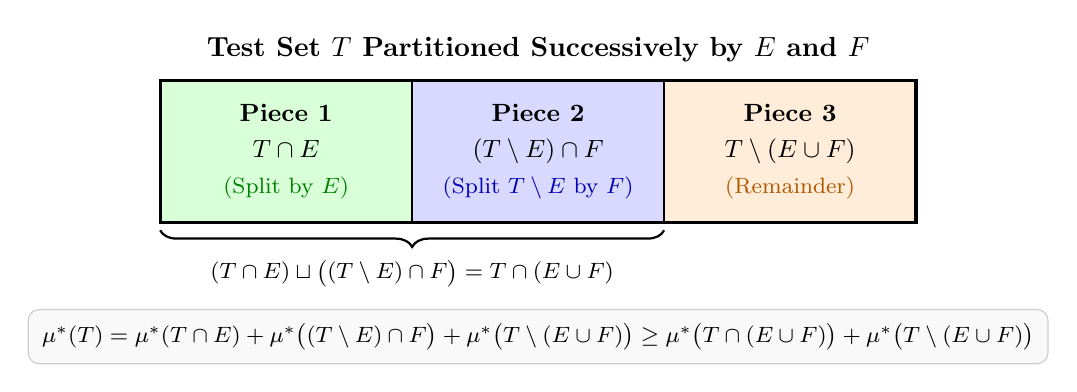
\begin{tikzpicture}[>=latex, font=\small]
  % Title above test set T
  \node[font=\bfseries] at (4.8, 3.0) {Test Set $T$ Partitioned Successively by $E$ and $F$};

  % Three contiguous, adjacent sub-rectangles partitioning T
  \fill[green!15] (0, 0.8) rectangle (3.2, 2.6);
  \fill[blue!15] (3.2, 0.8) rectangle (6.4, 2.6);
  \fill[orange!15] (6.4, 0.8) rectangle (9.6, 2.6);

  % Outer border of T and vertical partition lines
  \draw[very thick] (0, 0.8) rectangle (9.6, 2.6);
  \draw[thick] (3.2, 0.8) -- (3.2, 2.6);
  \draw[thick] (6.4, 0.8) -- (6.4, 2.6);

  % Piece labels
  \node[align=center] at (1.6, 1.7) {\textbf{Piece 1}\\[2pt] $T \cap E$\\[2pt] {\footnotesize\color{green!50!black}(Split by $E$)}};
  \node[align=center] at (4.8, 1.7) {\textbf{Piece 2}\\[2pt] $(T \setminus E) \cap F$\\[2pt] {\footnotesize\color{blue!70!black}(Split $T \setminus E$ by $F$)}};
  \node[align=center] at (8.0, 1.7) {\textbf{Piece 3}\\[2pt] $T \setminus (E \cup F)$\\[2pt] {\footnotesize\color{orange!70!black}(Remainder)}};

  % Curly underbrace spanning Pieces 1 and 2
  \draw[thick, decorate, decoration={brace, amplitude=6pt, mirror}] (0, 0.7) -- (6.4, 0.7)
    node[midway, below=7pt, font=\footnotesize\bfseries] {$(T \cap E) \sqcup \big((T \setminus E) \cap F\big) = T \cap (E \cup F)$};

  % Summary inequality box below underbrace
  \node[align=center, fill=gray!5, draw=gray!40, rounded corners, inner sep=5pt, font=\footnotesize] at (4.8, -0.65)
    {$\mu^*(T) = \mu^*(T \cap E) + \mu^*\big((T \setminus E) \cap F\big) + \mu^*\big(T \setminus (E \cup F)\big) \ge \mu^*\big(T \cap (E \cup F)\big) + \mu^*\big(T \setminus (E \cup F)\big)$};
\end{tikzpicture}
\end{document}
